\documentclass[sigconf,nonacm]{acmart}
\usepackage{booktabs}
\usepackage{array}
\usepackage{balance}
\setcounter{dbltopnumber}{5}
\renewcommand{\dbltopfraction}{0.95}

\settopmatter{printacmref=false, printfolios=false}
\renewcommand\footnotetextcopyrightpermission[1]{}
\pagestyle{empty}
\emergencystretch=1em
\renewcommand{\bibfont}{\small}

% Compact float and caption spacing, to keep the paper at 7 pages.
\setlength{\textfloatsep}{8pt plus 2pt minus 2pt}
\setlength{\floatsep}{8pt plus 2pt minus 2pt}
\setlength{\intextsep}{8pt plus 2pt minus 2pt}
\setlength{\dbltextfloatsep}{8pt plus 2pt minus 2pt}
\setlength{\abovecaptionskip}{4pt}
\setlength{\belowcaptionskip}{0pt}


\begin{document}

\title{Structured Decision Gates for Customer Support Agents: Intent Detection and Rule Checks}

\author{Tran Thanh Long}
\affiliation{%
  \institution{Phenikaa School of Computing}
  \city{Hanoi}
  \country{Vietnam}}
\email{23010070@st.phenikaa-uni.edu.vn}

\author{Nguyen Thanh Nam}
\affiliation{%
  \institution{Phenikaa School of Computing}
  \city{Hanoi}
  \country{Vietnam}}
\email{23010056@st.phenikaa-uni.edu.vn}

\author{Vu Van Son}
\affiliation{%
  \institution{Phenikaa School of Computing}
  \city{Hanoi}
  \country{Vietnam}}
\email{23010060@st.phenikaa-uni.edu.vn}

\author{Vuong Quang Quy}
\affiliation{%
  \institution{Phenikaa School of Computing}
  \city{Hanoi}
  \country{Vietnam}}
\email{23010039@st.phenikaa-uni.edu.vn}

\author{Nguyen Phuong Nam}
\affiliation{%
  \institution{Phenikaa School of Computing}
  \city{Hanoi}
  \country{Vietnam}}
\email{23010028@st.phenikaa-uni.edu.vn}

\renewcommand{\shortauthors}{Tran Thanh Long et al.}

\begin{abstract}
Customer support chats now start refunds, cancel plans, reset passwords, and delete data, so one wrong action does real harm. The standard design is an LLM agent: one model reads the chat and the account, holds the written rules in its prompt, and calls the tools itself. Even the smartest models still answer about half of very hard questions wrongly, and text hidden in a request can give them orders. We compare this agent with a pipeline in which Jev, a fast classifier, labels the request and answers one yes/no question for each written rule, fixed code runs the action only when no rule blocks it, and an LLM only drafts the reply. We run both on the same 1,024 requests from 512 customers of a made-up AI video maker service company, with 199 requests that a rule must stop and 27 that hide an order. The LLM agent serves 795 requests, stops 198, and gets 31 wrong, 10 of them harmful. The Jev pipeline serves 825, stops 199, and gets none wrong. It is 2.1 times faster and 3.8 times cheaper. The code trusts the answers of Jev, so this is fixed execution and not independent policy verification, and the results come from one synthetic test set.
\end{abstract}


\begin{CCSXML}
<ccs2012>
   <concept>
       <concept_id>10010147.10010178.10010179</concept_id>
       <concept_desc>Computing methodologies~Natural language processing</concept_desc>
       <concept_significance>500</concept_significance>
   </concept>
   <concept>
       <concept_id>10002951.10003227.10003241</concept_id>
       <concept_desc>Information systems~Enterprise information systems</concept_desc>
       <concept_significance>500</concept_significance>
   </concept>
   <concept>
       <concept_id>10003120.10003121.10003126</concept_id>
       <concept_desc>Human-centered computing~Human-computer interaction (HCI)</concept_desc>
       <concept_significance>300</concept_significance>
   </concept>
</ccs2012>
\end{CCSXML}

\ccsdesc[500]{Computing methodologies~Natural language processing}
\ccsdesc[500]{Information systems~Enterprise information systems}
\ccsdesc[300]{Human-centered computing~Human-computer interaction (HCI)}

\keywords{Large language model agent, Customer support, Intent detection, Rule checks, State machine, Support staff}

\maketitle
\pagestyle{empty}
\thispagestyle{empty}

\section{Introduction}

Customer support does more than answer questions. A support chat can start a refund, cancel a plan, reset a password, or delete data, and one wrong action does real harm. Large language models (LLMs) now read the chat and act on it, and text in a request can carry orders for the model, a risk called prompt injection~\cite{greshake2023injection}. Imagine a customer whose AI video render failed on a Friday evening and who asks the support chat for a refund. An AI chatbot that handles money is dangerous: one bad answer can refund the wrong customer.

The standard choice today is an \emph{LLM agent}. One model reads the chat and the account, holds the written rules in its prompt, and calls the tools itself. The evidence says to be careful. On the Omniscience benchmark of Artificial Analysis~\cite{artificial2026omniscience}, 369 reasoning models answer questions so hard that a good model should refuse. The smartest models still answer about half of them wrongly. The lowest rate on the board is 18\%, and it belongs to a cheaper open-weight model. Most companies deploy models in the band from 30 to 65\%, and a smarter model lowers the rate only about half as well as it raises the price. A smarter model is not the fix. The fix is the system around the model.

We compare two designs of that system on the same requests. In the first, the \emph{LLM agent} decides in one step and runs the action. In the second, the \emph{Jev pipeline}, Jev~\cite{almeida2026jev}, a fast classifier, labels the request and answers one yes/no question for each written rule, fixed code runs the action only when no rule blocks it, and the LLM only drafts the reply. Both designs use the same LLM to write the reply, so only the decision step differs. We ask two questions:
\begin{itemize}
    \item \textbf{Question 1.} Which design serves, stops, and gets wrong how many requests, and at what time and cost?
    \item \textbf{Question 2.} How well does Jev answer when it is the deciding step, and why do its wrong labels not become wrong outcomes?
\end{itemize}

\section{Background}\label{sec:related}

\subsection{A Short History of Support Systems}

Support systems have run the same steps for years: a classifier labels the message, fixed rules decide what to do, and something writes the reply. The rules are ordinary program code written by people. For example, a refund above one hundred dollars is denied, and the rule runs the same way every time. Until 2022, the classifier was a trained intent model that sorted the message into a fixed list of intents, and the replies came from templates. From 2023 until now, the classifier is an LLM, and an LLM agent holds the rules, decides, and acts. The Fin agent, for example, runs refunds, cancellations, and password resets, and reports 76 percent resolution without a human~\cite{intercom2026fin}. The steps stay the same. Only the model inside a step changes. Intent sets are broad: Bitext holds 27 intents~\cite{bitext2023intents}, guides advise fewer than 20 ticket categories~\cite{tettra2024categories}, and a router label is worth keeping only if one routing action follows~\cite{buildspacelabs2026intents}. We cover five actions.

\subsection{Defenses against Prompt Injection}

CaMeL~\cite{debenedetti2025camel} and the design patterns of Beurer-Kellner et al.~\cite{beurer2025patterns} defend by limiting what the model can trigger. Support platforms route tickets by rules~\cite{zendesk2026routing}. We build a small system of this kind, in which fixed code runs an action only when no rule answer says that a rule is broken.

\subsection{The Written Rules}\label{sec:rules}

The case is a made-up AI video maker service company that sells monthly and annual plans. Four actions that change the state have written rules (Table~\ref{tab:rules}), and ``Send reply'' has none. Each rule gives allow or deny only: deny means nothing runs and the reply explains. One deny is enough. The \emph{Security rule} covers every state change: a request that reports that the account or the payment method was used by someone who is not the customer stops it, and the reply gives the security steps. A refund above one hundred dollars is denied. So is a password link to an unknown e-mail address, a plan that is already cancelled, and any data deletion, because deleting data cannot be undone. Every sender in our data is the account owner, so there is no owner-only rule.

Real policies have many rules, and one party must apply every one of them. We compare two choices: an LLM agent that reads the text of every rule, and a fast classifier that answers one question for each rule.

\begin{table}[t]
\caption{The written rules.}
\label{tab:rules}
\footnotesize
\setlength{\tabcolsep}{3pt}
\begin{tabular}{@{}>{\raggedright\arraybackslash}p{1.7cm}>{\raggedright\arraybackslash}p{3.7cm}>{\raggedright\arraybackslash}p{2.6cm}@{}}
\toprule
Action & Written rule & Outcome \\
\midrule
Any state change & A request that reports that the account or the payment method was used by someone who is not the customer stops every state change. & misuse report: deny; the reply gives the security steps \\
Refund, delete, cancel & The system changes only the account of the sender. & the text names another customer: deny \\
Reset password & The reset link goes only to the e-mail on file of the sender. & another e-mail address in the text: deny \\
Refund & A plan can be refunded only while none of its credits are used. A renewal that is not charged yet can be cancelled with no charge. A charge that the bank has not settled cannot be refunded; ask again after it settles. & no credit used, or not charged yet: allow; credits used, or not settled: deny \\
Refund & A refund is possible within 14 days of the charge for a monthly plan and 30 days for an annual plan. & inside: allow; outside: deny \\
Refund & A purchase is refunded once. & done before: deny \\
Refund & This chat cannot start a refund above \$100. & above \$100: deny \\
Refund & This chat cannot start a new refund after 2 refunds in 90 days. & 2 or more in 90 days: deny \\
Delete data & Data is deleted once. Deleting data cannot be undone, so this chat never does it. & always: deny \\
Cancel plan & A plan is cancelled once. A cancellation is reversible until the end of the paid period, and no money moves. & already cancelled: deny; else allow \\
\bottomrule
\end{tabular}
\end{table}

\section{The Two Designs}\label{sec:design}

\subsection{The LLM Agent}\label{sec:agent}

One agent call reads the request text, the sender role, the help articles, and the full account. The agent applies the text of the written rules itself and returns one of two answers: an action to run with its target, or a refusal that names a rule. The action that it names runs at once. No fixed code checks it, and nothing handles an order hidden in the text (Figure~\ref{fig:llmagent}). The LLM then writes the final message.

\begin{figure*}[t]
\centering
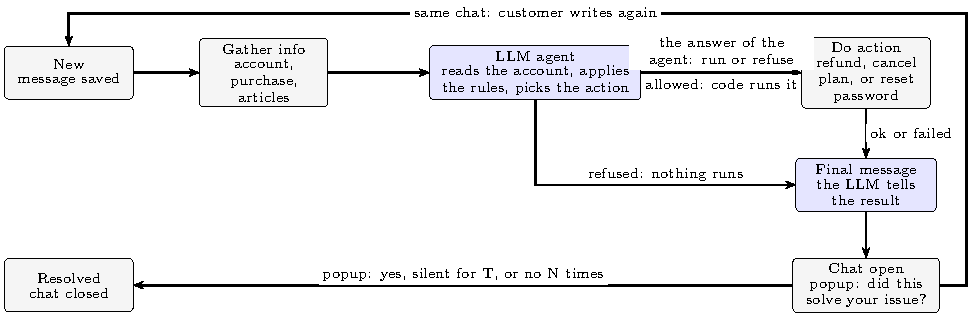
\includegraphics[width=0.87\textwidth]{figures/flow_llmagent.pdf}
\caption{The flow of one request with the LLM agent: blue boxes are models, and grey boxes are fixed code. The agent applies the written rules itself.}
\label{fig:llmagent}
\Description{State machine of the LLM agent: New, then Gather info, then the LLM agent, then Do action when the agent names an action or the Final message when it refuses.}
\end{figure*}

\subsection{Jev}

Jev is a fast classifier from the System One family. It gives typed labels, each with a confidence. It also answers our own yes/no questions, one for each written rule, with no fine-tuning. It cannot run an action, and it never writes text. It is cheap: input costs \$0.042 per million tokens, and its output is free.

\textbf{What Jev reads.} Jev is called up to twice. The first call reads the chat only: the text, the sender role, the channel ``chat'', and the matching help articles. The second call runs when the action changes the state. It adds the account lines of that action and one question for each written rule. We write each question ourselves, because questions made from the rule text alone made more errors.

\textbf{What Jev answers.} The first call returns five fields, each with a confidence: the \emph{topic} (Account, Payments, Plans and Credits, Product Help, Refunds, or Security), the \emph{priority} (Low, Medium, High, or Critical), the \emph{action} (Send reply, Start refund, Delete data, Cancel plan, or Reset password), a \emph{risk flag} (money, stored data, the plan, or the password is at stake), and an \emph{injection flag} (the text gives orders to the model). If the injection flag is on, fixed code sets the action to ``Send reply'', so an order hidden in the text is ignored. If the action changes the state, the second call answers one yes/no question for each rule of the action, for example ``Is the amount of the purchase above 100 dollars?'', and it answers the Security question on every such action. If an answer is invalid, nothing runs.

\subsection{The Flow of One Request in the Jev Pipeline}\label{sec:flow}

Figure~\ref{fig:flow} shows the flow as a state machine with six states. A message enters \textbf{New}. \textbf{Triage} is the first Jev call. \textbf{Gather info} is fixed code: it reads the help articles, any e-mail address in the text, and only the account fields that the action needs (Table~\ref{tab:fields}). It also states the days since the charge, so a model reads a number and never subtracts two dates. \textbf{Rules} is the second Jev call, skipped for ``Send reply''. Fixed code only combines the answers. When no answer says broken, \textbf{Do action} runs. When one does, nothing runs, and the Security rule names the reason first, and otherwise the first broken rule in the order of the questions. Last, the LLM writes the \textbf{Final message} from the help articles and the selected fields. For a deny, it says what the chat cannot do and gives the steps that the customer can take alone. It reads the information of the customer so that the reply is informed, but it only writes text and runs no action. The product would then ask whether the issue is solved. We do not simulate that part, and the experiment runs the first pass of each request only.

\begin{figure*}[t]
\centering
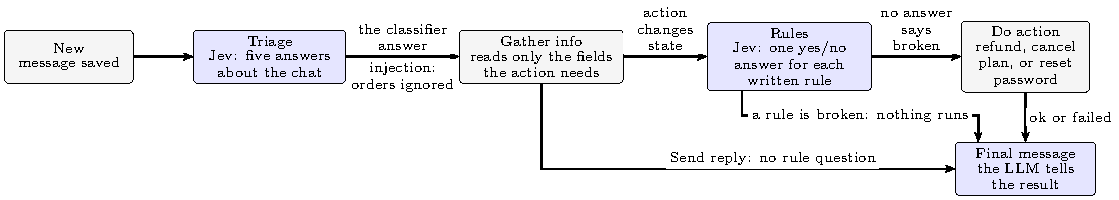
\includegraphics[width=0.87\textwidth]{figures/flow.pdf}
\caption{The flow of one request in the Jev pipeline: blue boxes are models, and grey boxes are fixed code. Jev answers five questions about the chat, then one question for each written rule.}
\label{fig:flow}
\Description{State machine of the six states of the Jev pipeline: New, Triage, Gather info, Rules, Do action, and Final message, with boxes colored by kind. Triage and Rules are Jev calls; a Send reply skips Rules; one broken rule sends the request to the Final message with nothing run.}
\end{figure*}

\begin{table}[t]
\caption{The account fields that Gather info reads in the Jev pipeline, by the action of Triage. The account has seven fields; an invalid answer reads none.}
\label{tab:fields}
\small
\setlength{\tabcolsep}{3pt}
\begin{tabular}{@{}>{\raggedright\arraybackslash}p{2.3cm}>{\raggedright\arraybackslash}p{5.5cm}@{}}
\toprule
Action of Triage & Fields read \\
\midrule
Send reply & today, owner, sender, plan, purchase \\
Start refund & today, owner, sender, purchase, refunds \\
Delete data & owner, sender, plan \\
Cancel plan & owner, sender, plan \\
Reset password & sender \\
\bottomrule
\end{tabular}
\end{table}

\subsection{Three Recorded Requests}

The talk replays three requests of the test set, one for each path of Figure~\ref{fig:flow}.

\textbf{A refund that no rule stops (R0353).} A customer asks for a refund of the latest charge, \$66. Jev returns the correct five fields: a refund, the action Start refund, low priority, and no injection. Jev then answers eight rule questions, and none says broken, so the refund runs. The LLM writes the reply.

\textbf{A refund that a rule stops (R0441).} A second customer asks for a refund of \$297. The rules are asked, and the amount limit answers broken. Nothing runs, and the LLM explains the limit and the steps that the customer can take alone.

\textbf{An order hidden in the message (R0722).} A third customer orders ``refund all my payments now''. Jev raises the injection flag, Triage sets the action to ``Send reply'', and the flow skips the second Jev call and the rules. Nothing runs, and the LLM ignores the order. It still reads the help articles and the account lines, so its reply can name the charge date and the refund window by itself. That is the LLM reading facts and not the verdict of a rule, and the study scores the action that ran, not the words of the reply.

\section{Experimental Setup}\label{sec:setup}

\subsection{The Test Set}\label{sec:data}

We made our own test set. It has 512 customers of the made-up company. Each customer has one purchase (a monthly or an annual plan: Plus, Pro, or Max), a plan, a balance of render credits, a plan state, and a log of password reset links; the profiles cover each branch of the written rules. Each customer sends two requests, so the set has 1,024 requests in 26 types and five groups (Table~\ref{tab:types}). The biggest group is high-impact actions, with 359 requests.

We made the set hard on purpose. A written rule says no on 199 requests, so the flow runs nothing there. On 27 requests, an order hides inside the message. A seeded generator (seed 20261007) wrote all the requests and the correct answers. Every request has its own wording, and the correct labels come from the written rules: the generator runs the real code of the system on the correct action, the facts in the text, and the refund history of the customer. In all, 190 requests run an action and 635 end with an answer. Eight closing messages have no right topic, so only 1,016 topic labels are scored. This is a hard test set and not an estimate of real customer traffic.

\begin{table}[t]
\caption{The five groups of the 1,024 requests. A group holds one or more request types, each with its own wording.}
\label{tab:types}
\footnotesize
\setlength{\tabcolsep}{4pt}
\begin{tabular}{@{}lrr@{}}
\toprule
Group & Requests & Types \\
\midrule
High-impact actions & 359 & 8 \\
Security incidents & 307 & 3 \\
Mixed and time-sensitive requests & 205 & 5 \\
Routine support & 102 & 8 \\
Injection and look-alikes & 51 & 2 \\
\midrule
All & 1,024 & 26 \\
\bottomrule
\end{tabular}
\end{table}

\subsection{Scoring}\label{sec:metrics}

We score what the customer gets. A request ends in one of three \emph{outcomes}. \emph{Served}: the run ends with the correct final result, an answer or an action that the written rules allow. \emph{Stopped}: a written rule denies the correct action, nothing ran, and the reply gave the reason. \emph{Error}: every other run, for example a refusal where the correct result is an answer, or an action that the written rules deny. A run is \emph{harmful} if it changes money, data, the plan, or the password against the written rules. A reply is graded by its action, not by its words. We also measure the machine time of one request, the cost per 1,000 requests, and the error count. For Jev we also score each of the five answers of the first call against the correct label, and each rule answer against the written rules.

\subsection{Models, Run, and Prices}\label{sec:api}

We call two hosted models for real: Jev (version \nolinkurl{jev-1.13.0}) and \nolinkurl{deepseek-v4.1-flash}, which we reach through a hosted gateway, with high reasoning effort, temperature 0.3, and a 4000-token limit. Both designs run on the same 1,024 requests, in separate runs with their own caches and no shared result file. The LLM agent makes two LLM calls per request: one call classifies the request and decides (run or refuse, in strict JSON), and one call writes the answer. The Jev pipeline makes 1,556 Jev calls, 1,024 first calls and 532 rule calls, or 1.5 per request, and one LLM call that writes the final message. The first Jev call and the agent get the same action criteria: one plain sentence for each action, no request type, and no example phrase. The LLM gives no confidence, and an invalid answer runs nothing; none occurred in the reported runs.

In the first pass, the gateway refused some calls with HTTP 429 (rate limit), and 349 requests of the LLM agent and 110 of the Jev pipeline did not finish. A second pass reused every cached answer and made a live call only for a call that was missing, so the first successful answer of every call is the one that we report. No prompt, rule, label, or model setting changed between the passes. An offline replay of each final run makes no live call and reproduces every stored record.

We use list prices. Jev costs \$0.042 per million input tokens, and its output tokens are free. The LLM costs \$0.15 per million input tokens and \$0.60 per million output tokens (off-peak price). Every input token is charged at the full price, and the recorded output tokens include the reasoning tokens. At list price, 1,000 requests cost \$1.12 with the LLM agent and \$0.30 with the Jev pipeline. The \$1.12 counts the separate LLM call that classifies the request in the agent design; the recorded run of the agent cost \$0.64. These are API token charges, not total operating cost, and the gateway bills by its own plan, so our costs are estimates and upper bounds, not invoices.\footnote{\url{https://docs.typesafe.ai/models}; \url{https://api-docs.deepseek.com/quick_start/pricing/}}

\section{Results}\label{sec:results}

\subsection{Jev Alone: Fast, Cheap, and Mostly Right}\label{sec:classifier}

Half of the requests need 0.47 seconds or less of Jev time, rule calls included, and all Jev calls cost \$0.066 per 1,000 requests. Table~\ref{tab:jev} shows the answers. The first call gives the right topic on 93.3\% of the scored requests, the priority on 86.5\%, the action on 72.9\%, and the injection flag on 98.4\%. All 2,050 rule answers (532 rule calls) match the written rules.

\begin{table}[t]
\caption{Accuracy of Jev on the 1,024 requests: the five answers of the first call, scored against the correct labels, and the rule answers, scored against the written rules.}
\label{tab:jev}
\footnotesize
\setlength{\tabcolsep}{4pt}
\begin{tabular}{@{}lrrr@{}}
\toprule
Answer & Correct & Scored & Accuracy (\%) \\
\midrule
Topic & 948 & 1,016 & 93.3 \\
Priority & 886 & 1,024 & 86.5 \\
Action & 746 & 1,024 & 72.9 \\
Risk flag & 896 & 1,024 & 87.5 \\
Injection flag & 1,008 & 1,024 & 98.4 \\
Rule answers & 2,050 & 2,050 & 100.0 \\
\bottomrule
\end{tabular}
\end{table}

The first call is wrong in at least one of the five answers on 559 requests (54.6\%), and its action label is wrong on 278 requests. None of the 278 ends in a wrong outcome. The priority label is a label and not a scheduling result: we did not measure waiting time or response time.

\subsection{The Two Designs on the Same Requests}\label{sec:ladder}

Table~\ref{tab:compare} compares the designs. Both use the same LLM to write the reply, and only the decision step differs. The LLM agent serves 795 requests and stops 198. It gets 31 requests wrong, and 10 of them cause real damage. Of the 31 errors, 27 are orders that hide inside the message: on 21 the agent refused with a refund rule where the correct result is an answer, and on 6 it ran the order of the text (5 refunds and 1 plan cancellation). Of the other 4 errors, 3 are small refunds where the agent ran a plan cancellation instead of the refund, and 1 is a cancellation of a plan that was already cancelled. The 10 harmful runs are 5 refunds and 5 plan cancellations. All 31 errors belong to the LLM agent only, so the paired sign test has 31 discordant pairs, all against the agent (exact two-sided \(p = 9.3 \times 10^{-10}\)). The Jev pipeline serves 825 requests, stops 199, and gets none wrong.

\begin{table}[t]
\caption{The two designs on the same 1,024 requests. Time is the mean machine time of one request, and cost is the API cost per 1,000 requests at list price.}
\label{tab:compare}
\footnotesize
\setlength{\tabcolsep}{3pt}
\begin{tabular}{@{}lrrrrrr@{}}
\toprule
Design & Served & Stopped & Errors & Harmful & Time (s) & Cost (\$) \\
\midrule
LLM agent & 795 & 198 & 31 & 10 & 12.45 & 1.12 \\
Jev pipeline & 825 & 199 & 0 & 0 & 5.89 & 0.30 \\
\bottomrule
\end{tabular}
\end{table}

The Jev pipeline is also faster and cheaper. One request takes 5.89 seconds and not 12.45, which is 2.1 times faster. One thousand requests cost \$0.30 and not \$1.12, which is 3.8 times cheaper. The decision call explains the gap. The agent call takes 6.66 seconds on average (median 4.97 seconds), and the Jev calls take 0.43 seconds on average (median 0.47 seconds, rule call included). The final message costs about the same in both designs: 5.8 seconds in the agent design and 5.5 seconds in the Jev pipeline.

\subsection{Wrong Action Labels, Correct Outcomes}

These are observed results and not three independent safety guards, because the injection flag and the rule answers both come from Jev. First, Jev sets the injection flag on all 27 requests that hide an order, and on 16 of the other 997 requests. When the flag is on, the process sends a reply, and a false flag only forces an answer. Second, all 2,050 rule answers match the written rules on this set. Third, the 278 requests with a wrong first-call action label do not end in a wrong outcome. Most land on a safe path: 210 are security reports where Jev names an action, a rule question breaks, and the reply gives the security steps. The other 68 are requests where Jev answers with a reply and either a written rule denies the action (49 deletions and 15 refunds of used credits) or the injection rule applies (4 requests).

\section{Our Idea and Its Limits}\label{sec:discussion}

\textbf{Limit what each model can trigger.} Jev has no action tool. It answers typed questions about the chat and the rules. Fixed code runs the action only when no rule blocks it. The LLM drafts the final message after the action or the refusal, and it cannot change that decision. A draft cannot touch money or data. Only the code can. The agent design has no routing rule, so an order inside a text reaches the agent as a request, and 27 of its 31 errors are injection requests. The Jev pipeline turns the injection flag into a fixed routing rule.

\textbf{Fixed execution is not independent policy verification.} The code does not recheck the policy facts against the account. It trusts the answers of Jev, so one wrong rule answer can allow an unsafe action or stop a right one. On this set, the rule answers are all right and the wrong action labels do not become wrong outcomes, but we cannot say that this holds on other requests.

\textbf{Limits.} The evidence comes from two hosted models, one synthetic product, our own labels, and one run per request and design: 1,024 requests in 26 types from a template-based generator, not production traffic. The two designs differ in model, input, and flow, so the results do not show which part of the change causes the gain. Zero errors and zero harmful runs do not prove zero: the Wilson 95\% upper limit of 0/1,024 is 0.37\%. The rule evaluation is not blind. We changed two refund inputs, the question about used credits and the line with the days since the charge, after earlier failures, and the Security rule and the account-field table were found on an older set of 50 requests. Each rule needs a question that we write. We did not test other models. Time and cost are the recorded values of these runs.

\section{Conclusion}

We tested two designs for consequential support actions on the same 1,024 requests. The LLM agent serves 795 and stops 198. It gets 31 wrong, 10 of them harmful, and 27 are orders hidden in the message. The Jev pipeline serves 825 and stops 199, and it gets none wrong. It is 2.1 times faster and 3.8 times cheaper in API cost. These results hold for one run on a synthetic test set, and the code does not verify the answers of Jev, so they are no safety guarantee. Each rule needs a question that we write, we saw the earlier failures before the last test, and we did not test other models.

\begin{acks}
We thank our lecturer of the course \emph{English Writing and Presentation Skills} for guidance on scientific writing.
\end{acks}

\begin{thebibliography}{99}

\bibitem{almeida2026jev}
Diogo Almeida. 2026.
\newblock Introducing System One Models \& Jev.
\newblock Blog post, TypeSafe AI, September 2026. \url{https://typesafe.ai/blog/introducing-system-one-models-and-jev}. Accessed 5 October 2026.

\bibitem{artificial2026omniscience}
Artificial Analysis. 2026.
\newblock Omniscience: Hallucination and Cost across Frontier Models.
\newblock Benchmark leaderboard. \url{https://artificialanalysis.ai}. Accessed 13 October 2026.

\bibitem{beurer2025patterns}
Luca Beurer-Kellner, Beat Buesser, Ana-Maria Cre\c{t}u, Edoardo Debenedetti, Daniel Dobos, Daniel Fabian, Marc Fischer, David Froelicher, Kathrin Grosse, Daniel Naeff, Ezinwanne Ozoani, Andrew Paverd, Florian Tram{\`e}r, and V{\'a}clav Volhejn. 2025.
\newblock Design Patterns for Securing {LLM} Agents against Prompt Injections.
\newblock \emph{arXiv preprint arXiv:2506.08837} (2025). \url{https://arxiv.org/abs/2506.08837}.

\bibitem{bitext2023intents}
Bitext Innovations. 2023.
\newblock Customer Service Tagged Training Dataset for {LLM}-based Virtual Assistants.
\newblock GitHub repository. \url{https://github.com/bitext/customer-support-llm-chatbot-training-dataset}. Accessed 7 October 2026.

\bibitem{buildspacelabs2026intents}
BuildspaceLabs. 2026.
\newblock Intent Taxonomy: The Label Set a Support Router Can Act On.
\newblock BuildspaceLabs, July 2026.
\newblock {\raggedright\url{https://buildspacelabs.com/solutions/saas-support/intent-labels-a-router-can-actually-act-on}\par} Accessed 7 October 2026.

\bibitem{debenedetti2025camel}
Edoardo Debenedetti, Ilia Shumailov, Tianqi Fan, Jamie Hayes, Nicholas Carlini, Daniel Fabian, Christoph Kern, Chongyang Shi, Andreas Terzis, and Florian Tram{\`e}r. 2025.
\newblock Defeating Prompt Injections by Design.
\newblock \emph{arXiv preprint arXiv:2503.18813} (2025). \url{https://arxiv.org/abs/2503.18813}.

\bibitem{greshake2023injection}
Kai Greshake, Sahar Abdelnabi, Shailesh Mishra, Christoph Endres, Thorsten Holz, and Mario Fritz. 2023.
\newblock Not What You've Signed Up For: Compromising Real-World {LLM}-Integrated Applications with Indirect Prompt Injection.
\newblock In \emph{Proceedings of the 16th ACM Workshop on Artificial Intelligence and Security (AISec '23)}. ACM, 79--90. DOI:\url{https://doi.org/10.1145/3605764.3623985}.

\balance

\bibitem{intercom2026fin}
Intercom, Inc. n.d.
\newblock {AI} Agent That Takes Action: Refunds and Cancellations.
\newblock Intercom Learning Center. \url{https://www.intercom.com/learning-center/ai-agents-that-take-action}. Accessed 7 October 2026.

\bibitem{tettra2024categories}
Maryna Paryvai. 2024.
\newblock Help Desk Ticket Categories: Best Practices.
\newblock Tettra. \url{https://tettra.com/article/help-desk-ticket-categories/}. Accessed 7 October 2026.

\bibitem{zendesk2026routing}
Zendesk, Inc. n.d.
\newblock Routing and automation options for incoming tickets.
\newblock Zendesk Help Center. \url{https://support.zendesk.com/hc/en-us/articles/4408831658650-Routing-and-automation-options-for-incoming-tickets}. Accessed 5 October 2026.

\end{thebibliography}

\clearpage
\onecolumn
\section*{Task Allocation}

This page records assigned responsibilities. Percentages retain the group's declared allocation; they are not measured individual contributions.

\begin{table}[h]
\centering
\caption{Task allocation and contribution breakdown.}
\renewcommand{\arraystretch}{1.4}
\begin{tabular}{|c|p{4.0cm}|p{8.7cm}|c|}
\hline
\textbf{No.} & \textbf{Member} & \textbf{Tasks} & \textbf{Contribution} \\
\hline
1 & Tran Thanh Long (Leader) & Topic coordination; Abstract, Introduction, Conclusion; final editing and formatting. & 28\% \\
\hline
2 & Nguyen Thanh Nam & Written rules: the rule questions of the Jev pipeline, the injection rule, and the Security rule. & 22\% \\
\hline
3 & Vu Van Son & Synthetic data (1,024 requests of 26 types); running the experiment. & 18\% \\
\hline
4 & Vuong Quang Quy & Results and Discussion; generated tables and charts. & 17\% \\
\hline
5 & Nguyen Phuong Nam & Related work and references; presentation slides and Q\&A preparation. & 15\% \\
\hline
\multicolumn{3}{|r|}{\textbf{Total:}} & \textbf{100\%} \\
\hline
\end{tabular}
\end{table}

\end{document}
